\documentclass[12pt]{article}
\usepackage{amsmath}
\usepackage{hyperref}
\usepackage{tikz} % for ARS drawings

\title{CPSC 354 Report}
\author{Jonathan Karam }
\date{\today}

\begin{document}

\maketitle

\begin{abstract}
This report is for the assingment hw1 of CPSC 354. With the primary goal of using git as well as LaTex and practice. I will explain the MU puzzle explain the MU puzzle.
\end{abstract}

\tableofcontents

\section{Introduction}
This report will expand as the semester goes on, for now it will cover homework 1

\section{Week by Week}

\subsection{Week 1}

\subsubsection*{Homework: The MU Puzzle}

The MU puzzle is a small game made up of letters and rules. You start with the
string \texttt{MI}. The main challenge seeing if you can turn it into the string
\texttt{MU} by following a few rules

\begin{enumerate}
  \item If a string ends with \texttt{I}, you can add a \texttt{U} at the end.  
        Example: \texttt{MI} $\to$ \texttt{MIU}.
  \item If you have a string that begins with \texttt{M}, you can copy everything
        after the \texttt{M} and put it again.  
        Example: \texttt{MIU} $\to$ \texttt{MIUIU}.
  \item If you see \texttt{III} anywhere, you can change it into a \texttt{U}.  
        Example: \texttt{MIII} $\to$ \texttt{MU}.
  \item If you see \texttt{UU}, you can remove it.  
        Example: \texttt{MUUU} $\to$ \texttt{MU}.
\end{enumerate}

At first it seems like you should be able to get from \texttt{MI} to
\texttt{MU}, but you can't. The reason is that the number of
\texttt{I}'s never works out in the right way. You start with one \texttt{I}.
Using the rules, you can never get rid of all the \texttt{I}'s. To make
\texttt{MU}, you would need zero \texttt{I}'s, but that is not possible.  

The lesson is that even with very simple rules, there can be hidden limits on what you can do.

\section{Conclusion}
The MU puzzle shows that rules can look simple, but still create pretty deep limits.
This makes it a good example on how formal systems work.

\newpage
\section{Homework 2 Rewriting ARS Pictures}

Below you will see the directed graphs for the seven ARS's. Nodes are the elements of A and arrows are the pairs in R.

\subsection{1: $A=\{\}$}
\begin{tikzpicture}
  %empty
\end{tikzpicture}

\subsection{2: $A=\{a\},\ R=\{\}$}
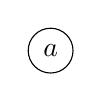
\begin{tikzpicture}
  \node[circle,draw] (a) at (0,0) {$a$};
\end{tikzpicture}

\subsection{3: $A=\{a\},\ R=\{(a,a)\}$}
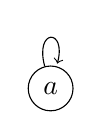
\begin{tikzpicture}
  \node[circle,draw] (a) at (0,0) {$a$};
  \draw[->] (a) edge[loop above] (a);
\end{tikzpicture}

\subsection{4: $A=\{a,b,c\},\ R=\{(a,b),(a,c)\}$}
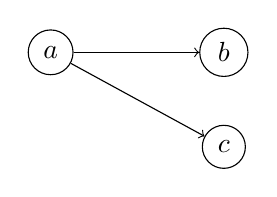
\begin{tikzpicture}
  \node[circle,draw] (a) at (0,0) {$a$};
  \node[circle,draw] (b) at (2.2,0) {$b$};
  \node[circle,draw] (c) at (2.2,-1.2) {$c$};
  \draw[->] (a) -- (b);
  \draw[->] (a) -- (c);
\end{tikzpicture}

\subsection{5: $A=\{a,b\},\ R=\{(a,a),(a,b)\}$}
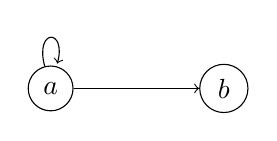
\begin{tikzpicture}
  \node[circle,draw] (a) at (0,0) {$a$};
  \node[circle,draw] (b) at (2.2,0) {$b$};
  \draw[->] (a) edge[loop above] (a);
  \draw[->] (a) -- (b);
\end{tikzpicture}

\subsection{6: $A=\{a,b,c\},\ R=\{(a,b),(b,b),(a,c)\}$}
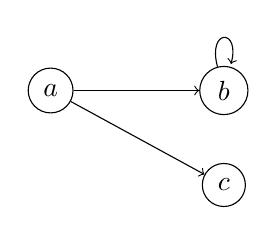
\begin{tikzpicture}
  \node[circle,draw] (a) at (0,0) {$a$};
  \node[circle,draw] (b) at (2.2,0) {$b$};
  \node[circle,draw] (c) at (2.2,-1.2) {$c$};
  \draw[->] (a) -- (b);
  \draw[->] (a) -- (c);
  \draw[->] (b) edge[loop above] (b);
\end{tikzpicture}

\subsection{7: $A=\{a,b,c\},\ R=\{(a,b),(b,b),(a,c),(c,c)\}$}
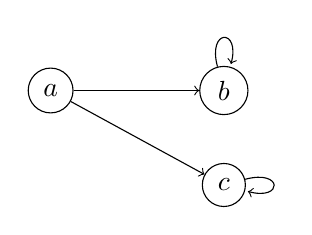
\begin{tikzpicture}
  \node[circle,draw] (a) at (0,0) {$a$};
  \node[circle,draw] (b) at (2.2,0) {$b$};
  \node[circle,draw] (c) at (2.2,-1.2) {$c$};
  \draw[->] (a) -- (b);
  \draw[->] (a) -- (c);
  \draw[->] (b) edge[loop above] (b);
  \draw[->] (c) edge[loop right] (c);
\end{tikzpicture}

\end{document}
